\addcontentsline{toc}{section}{Introduction}
\section*{Introduction}
Dans ce chapitre, nous présentons les différentes fonctionnalités de notre système.   Les résultats obtenus sont assez satisfaisants. Ces résultats encourageants montrent des possibilités d'adoption de la reconnaissance de locuteur dans divers domaines, tels que la sécurité biométrique pour l'identification de personnes, la surveillance des appels téléphoniques, les centres d'appels et les interactions vocales dans les voitures connectées. Dans ce chapitre, nous repréciserons le cadre d’étude de notre système, ainsi que lesdits résultats, obtenus à l’issue de l’implémentation. 

\section{Présentation du cadre d’étude}
Le présent système mis sur pieds a pour but la reconnaissance de locuteur.
La reconnaissance de locuteur est une application de l'intelligence artificielle (IA) qui vise à identifier et à authentifier une personne en fonction de sa voix. 
Cette technologie peut être utilisée dans différents contextes tels que la sécurité, l'assistance vocale, la gestion de la relation client, etc. 
l’IA pourra être déployée et mise à la disposition des services de la criminologie pour servir lors des enquêtes judiciaires pour identifier des individus. 
Elle pourra également servir à sécuriser les systèmes en implémentant un MFA (Multi-Factor Authentication) afin d’accroitre la sécurité des systèmes.


\section{Résultats obtenus}
Nous rappelons que la génération de nos modèles, à partir des données d’apprentissage a été possible grâce au service cloud de Google Colaboratory . Celui-ci est un outil intuitif donnant accès à des ressources informatiques permettant de travailler sur des projets en science des données. Par la suite ces modèles ont été sauvegardé sur Cloud Storage afin d’alimenter notre application Django qui offrira les APIs pour les opérations d’identification et d’authentification.
L'utilisation de l'IA pour la reconnaissance de locuteur a connu une avancée significative au cours des dernières années grâce à l'amélioration des algorithmes d'apprentissage automatique et de traitement du signal vocal. Les résultats obtenus sont encourageants et permettent d'identifier un locuteur avec une précision élevée.
Les tests réalisés sur des enregistrements de voix ont montré que l'IA est capable de reconnaître un locuteur avec une précision pouvant varier en fonction de la qualité de l'enregistrement, du bruit ambiant et de la durée de la parole. 

\subsection{liste des locuteurs}
La figure suivante présente la liste des locuteurs. Dans notre architecture, nous les avons appelé POI (Person Of Interest). 

\begin{figure}[h]
	\centering
	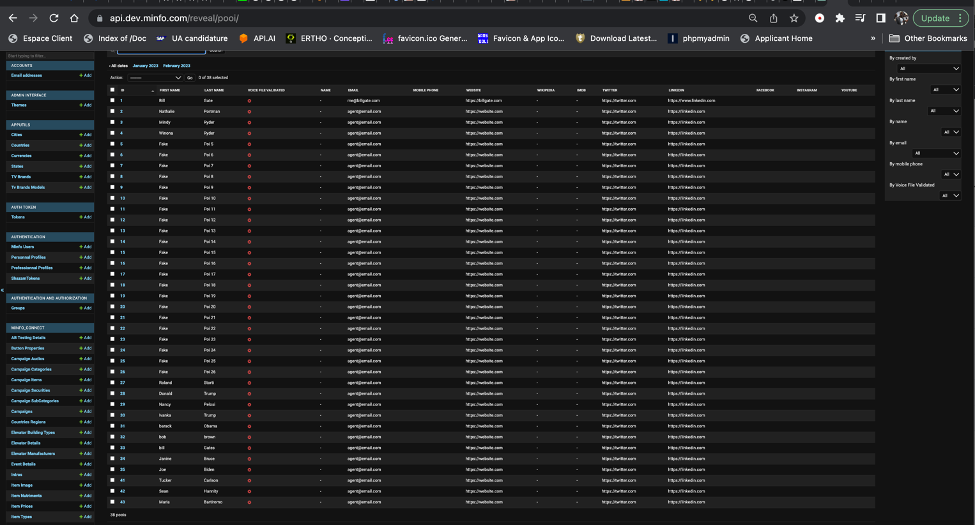
\includegraphics[width=1\textwidth]{4chap1}
	\caption{Liste des POI}
	\label{fig:4chap1}
\end{figure}
A partir de cette page nous pouvons facilement étendre la liste, ajouter des empreintes vocales pour les différents POIs.

\subsection{mise à jour du model}
Après l’entrainement sur Google Colab, le model est exporté vers Cloud Storage pour usage ultérieure.

\begin{figure}[h]
	\centering
	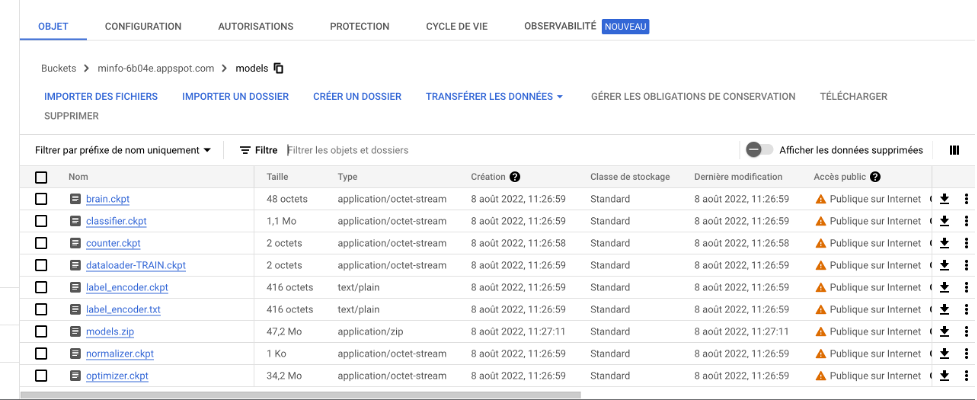
\includegraphics[width=1\textwidth]{4chap2}
	\caption{Meilleure modèle sauvegardé sur Cloud Storage}
	\label{fig:4chap2}
\end{figure}
Afin de récupérer ce model et l’utiliser en production dans notre projet Django, nous appelons la route  \textbf{api/speaker/updatemodel}

\begin{figure}[h]
	\centering
	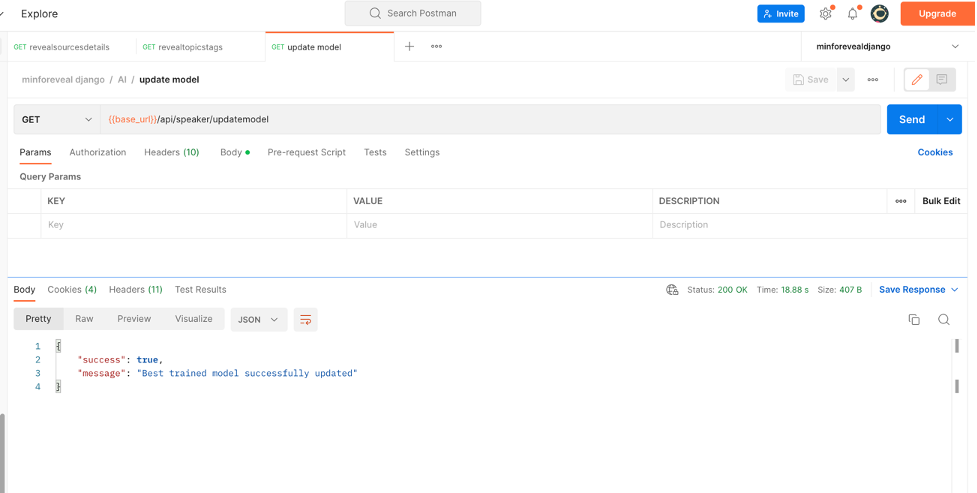
\includegraphics[width=1\textwidth]{4chap3}
	\caption{récupération du meilleur modèle}
	\label{fig:4chap3}
\end{figure}

\subsection{Identification de locuteur}
L’identification répond à la question : « Qui est cette personne ? ». Elle consiste à vérifier dans notre base de données à qui correspond une empreinte vocale.  

\begin{figure}[h]
	\centering
	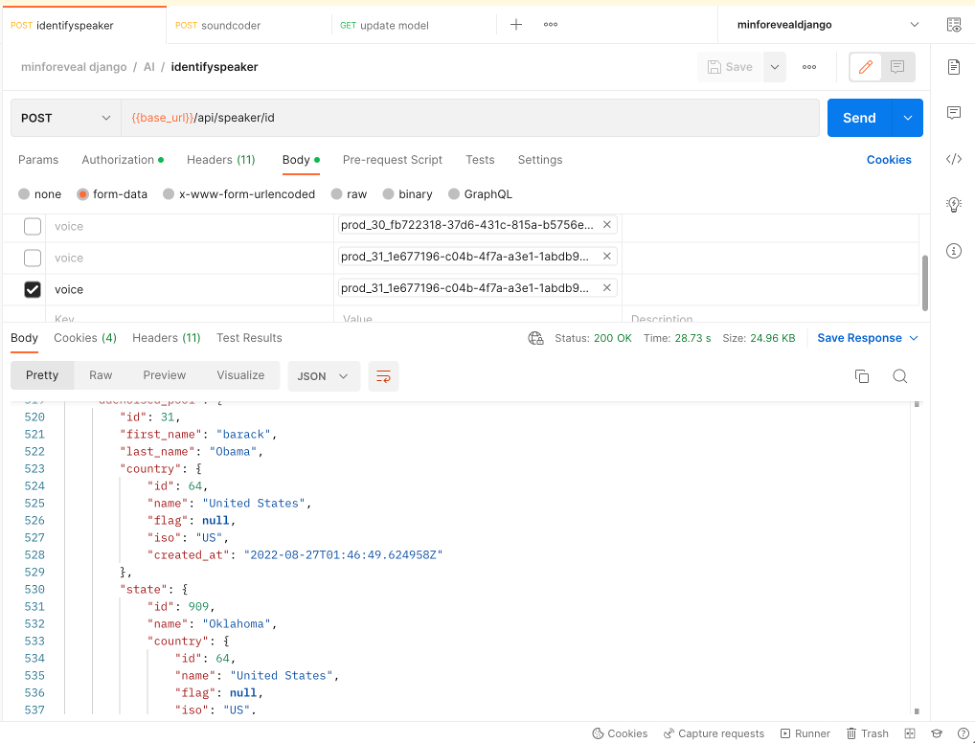
\includegraphics[width=1\textwidth]{4chap4}
	\caption{Identification de locuteur}
	\label{fig:4chap4}
\end{figure}
\textbf{Route:  /api/speaker/id}
\\\textbf{Requête : POST}
\\\textbf{Paramètre : voice(le fichier vocal)}
\\\textbf{Le locuteur doit être dans la liste des POI.}

\subsection{authentification de locuteur}
L’authentification permet de répondre à la question : « Le locuteur est-il vraiment celui qu’il prétend être ? ». Pour cet API on n’a pas besoin d’avoir les empreintes vocales du locuteur. Ainsi la plateforme qui intègre l’API peut conserver ses empreintes sur ses serveurs privés cela resoud en même temps les problématiques de privilèges d’accès aux données, de sécurités et de confidentialité.
\\\textbf{route  /api/speaker/match}
\\\textbf{Requête : POST}
\\\textbf{Paramètre : voice1 et voice2(le fichier vocal empreinte et le fichier vocale enregistré à l’authentification)}
\\\textbf{Le locuteur n’a pas besoin d’être enregistré dans la base des POI.}

\begin{figure}[h]
	\centering
	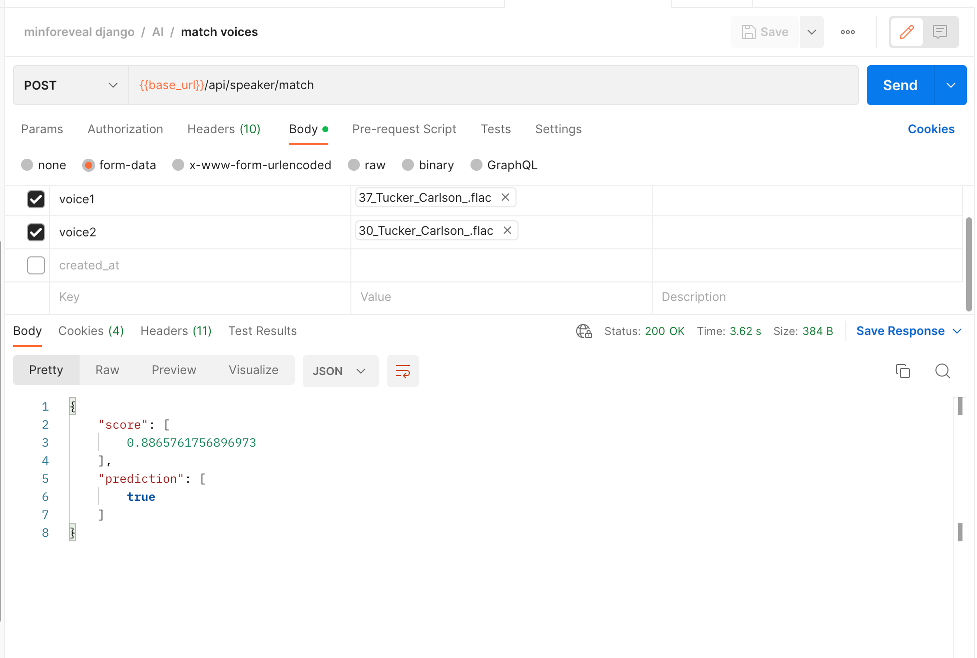
\includegraphics[width=1\textwidth]{4chap5}
	\caption{Identification de locuteur}
	\label{fig:4chap5}
\end{figure}

\paragraph{}La prédiction représente le résultat de l’authentication :

\begin{itemize}
    \item True signifie que l’utilisateur est bien celui qu’il prétend être
    \item False signifie que l’utilisateur n’est pas le bon, c’est-à-dire que la voix ne correspond pas à l’empreinte vocale.
\end{itemize}

\subsection{Analytic des connexions}
Nous avons mise en place un service d’analytique pour le suivi et l’utilisation du système. Il enregistre la date, le fichier vocal et le résultat du scan. 


\begin{figure}[h]
	\centering
	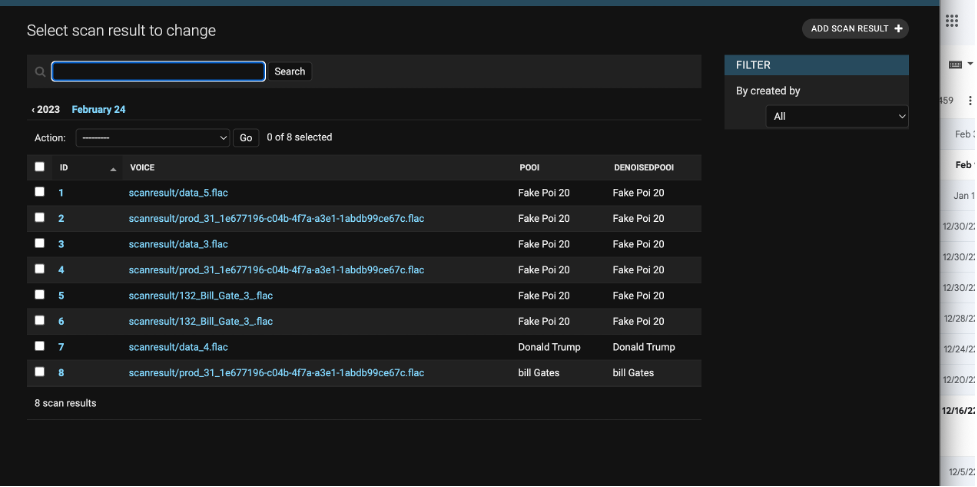
\includegraphics[width=1\textwidth]{4chap6}
	\caption{Identification de locuteur}
	\label{fig:4chap6}
\end{figure}

\section{avantage de notre architecture}
Le TDNN (Time Delay Neural Network) est l’architecture de réseau de neurones artificiels qui a été utilisée dans. Le cas de notre étude pour la reconnaissance de locuteur. Concernant ses avantages, nous pouvons citer :
\begin{itemize}
    \item Le TDNN est relativement rapide à entraîner et à utiliser une fois qu'il a été entraîné.
    \item Les TDNN peuvent prendre en compte les caractéristiques temporelles des signaux acoustiques. En effet, les TDNN sont capables de prendre en compte les données d'entrée passées et présentes, ce qui est important pour la reconnaissance de locuteur.
    \item Les TDNN peuvent être utilisés pour extraire des caractéristiques discriminantes des signaux acoustiques. Les TDNN peuvent apprendre des caractéristiques complexes des signaux acoustiques, ce qui est important pour la reconnaissance de locuteur.
    \item Les TDNN peuvent être entraînés sur de grandes quantités de données. Les TDNN sont capables d'apprendre à partir de grandes quantités de données, ce qui est important pour la reconnaissance de locuteur.
\end{itemize}

\section{Les limites de notre architecture}
Il convient de noter que les inconvénients du TDNN pour la reconnaissance de locuteurs peuvent varier en fonction du contexte d'utilisation et des caractéristiques des données de parole utilisées pour l'entraînement et le test.
Les TDNN peuvent être sensibles aux variations de conditions d'enregistrement. Les TDNN peuvent être affectés par des facteurs tels que le bruit de fond, la qualité de l'enregistrement, la distance entre le locuteur et le microphone, etc.
Les TDNN peuvent nécessiter une grande quantité de données d'entraînement. Pour obtenir des performances de reconnaissance de locuteur élevées, il peut être nécessaire de disposer d'une grande quantité de données d'entraînement.
Les TDNN peuvent nécessiter une puissance de calcul importante. L'entraînement et l'utilisation de TDNN peut être coûteux en termes de puissance de calcul, surtout lorsqu'il s'agit de grandes quantités de données.

\addcontentsline{toc}{section}{Conclusion}
\section*{Conclusion}
Dans ce chapitre, nous avons présenté les résultats obtenus à travers quelques figures présentants l’utilisation de nos different APIs.
Dans le cas où l'IA est bien entraînée avec des données de haute qualité et utilisée dans un contexte approprié, elle peut fournir une reconnaissance de locuteur précise et fiable. Cela peut être utile dans diverses applications, telles que la sécurité de l'authentification vocale, l'analyse de la parole pour la recherche et la reconnaissance de locuteur dans les applications de communication.
Cependant, l'utilisation d'une IA pour la reconnaissance de locuteur peut également soulever des préoccupations en matière de vie privée et de sécurité. Si les données vocales utilisées pour entraîner l'IA sont mal protégées, elles peuvent être utilisées pour identifier les utilisateurs sans leur consentement, ou même être utilisées à des fins malveillantes. Il est donc important de prendre des mesures pour protéger la vie privée des utilisateurs et de veiller à ce que l'utilisation de l'IA pour la reconnaissance de locuteur soit justifiée et éthique. C’est pour ça que notre implémentation de l’authentification renécessite pas une sauvegarde par notre système des empreinte vocaux. 
En résumé, l'utilisation d'une IA pour la reconnaissance de locuteur peut être utile dans certains contextes, mais elle nécessite une attention particulière pour garantir la précision, la fiabilité et la protection de la vie privée des utilisateurs.
